\section{试验和结果}
\subsection{实验环境}
本文实验的训练和测试均搭建于Linux操作系统,版本为Ubuntu20.06 LTS。使用的处
理器为Intel CORE I7,开发工具为 Ananconda3、python3.8、Pycharm。模型的开发基于
Simpy 4.0.1、Pyomo 6.5.0、gurobipy 10.0框架。

\subsection{数据准备}
解决排队问题首先要根据原始资料作出乘客到达间隔和服务时间的经验分布,根据以往经验,校园公交车站客流呈周期性变化,
选择文德楼北上行线车站实地统计,该车站位于校门、宿舍楼、主教学楼连接处的枢纽位置,客流量较有代表性,采样地点如图~\ref{fig31}~。
\\
\begin{figure}[htbp!]
    \centering
    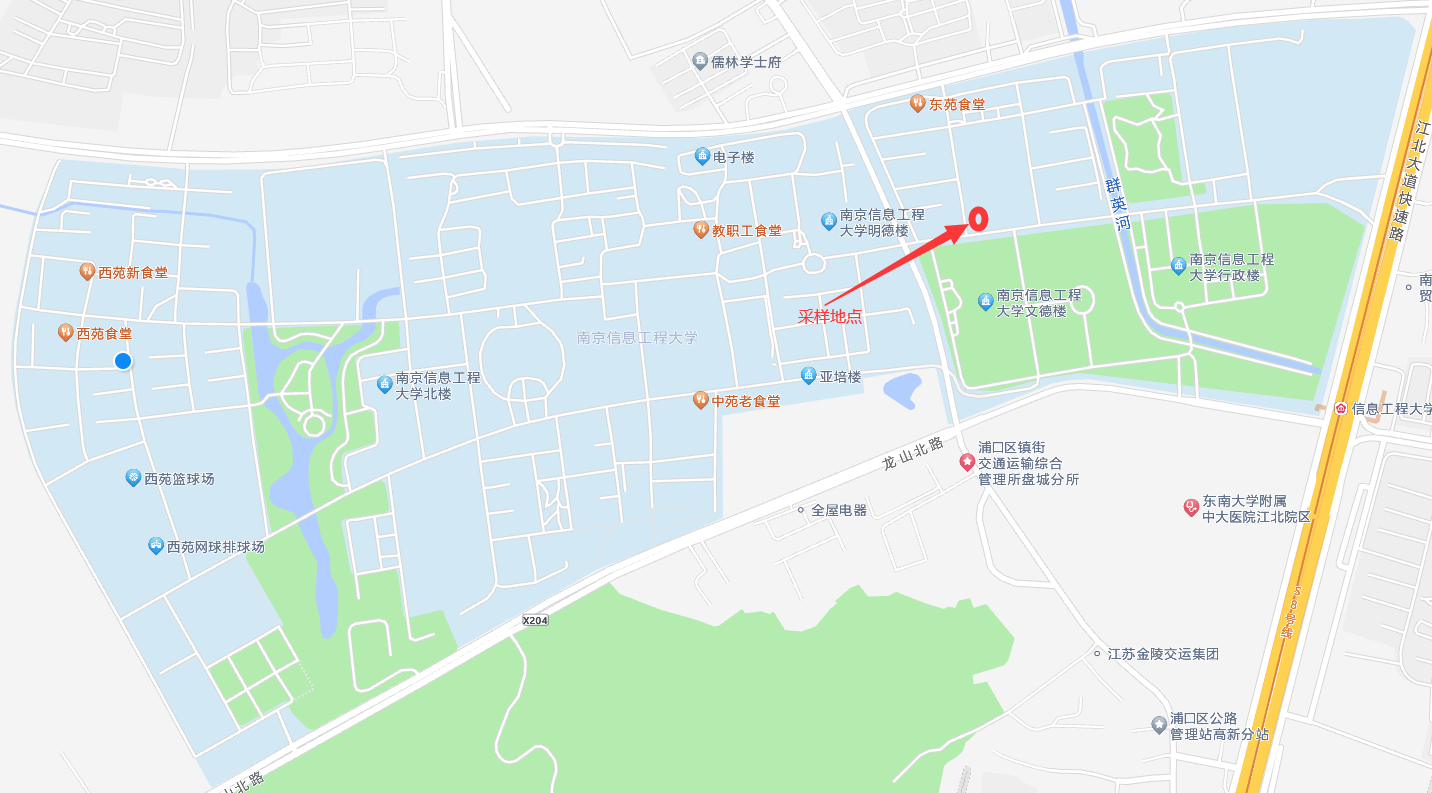
\includegraphics[width=0.7\textwidth]{figs/chap03/map.png}
    \caption{采样地点}
    \label{fig31}
\end{figure}

原始数据记载乘客到达时刻和对应的等待时间,以 $\tau_i$ 表示第i个乘客到达的时刻,以s表示等待时间可以得出相继到达时间 $t_i \left(t_i = \tau_{i+1} - \tau_i\right)$ 和等待时间 $w_i$,
它们的关系如图~\ref{fig32}~。

\begin{figure}[htbp!]
    \center
    \subfigure[$w_i + s_i - t_i > 0$]{\label{queue1}
    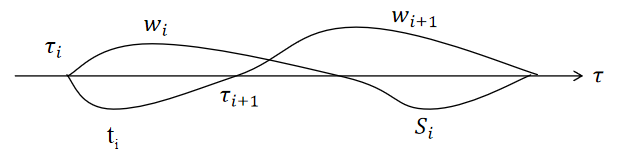
\includegraphics[width=0.7\textwidth]{figs/chap03/queue1.png}
    }
    \\
    \subfigure[$w_i + s_i - t_i < 0$]{\label{queue2}
    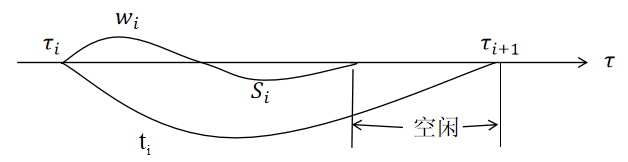
\includegraphics[width=0.7\textwidth]{figs/chap03/queue2.png}
    }
    \caption{相继到达的间隔时间和排队等待时间关系示意图}\label{fig32}
\end{figure}

由图~\ref{fig32}~可以得到如下关系:

间隔\quad \quad \quad \quad$t_i = \tau_{i+1} - \tau_i$

等待时间 \quad \quad 
$
w_{i+1} = 
\begin{cases}
    w_i + s_i - t_i,\quad w_i + s_i - t_i > 0
    \\
   0, \qquad \qquad \quad w_i + s_i - t_i < 0
\end{cases}
$


% \begin{figure}[htbp!]
%     \center
%     \subfigure[$w_i + s_i - t_i > 0$]{\label{queue1}
%     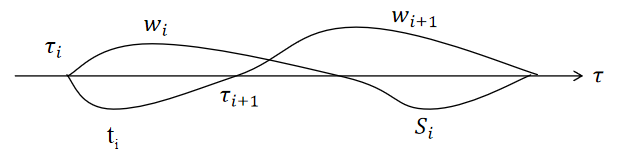
\includegraphics[width=0.5\textwidth]{figs/chap03/queue1.png}
%     }
%     \\
%     \subfigure[$w_i + s_i - t_i < 0$]{\label{queue2}
%     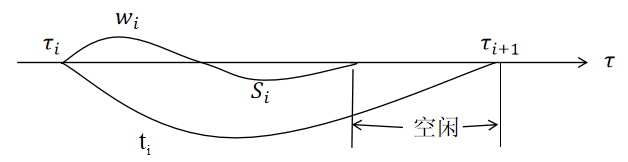
\includegraphics[width=0.5\textwidth]{figs/chap03/queue2.png}
%     }
%     \caption{相继到达的间隔时间和排队等待时间关系示意图}\label{fig32}
% \end{figure}

由图~\ref{fig32}~可以得到如下关系:

间隔\quad \quad \quad \quad$t_i = \tau_{i+1} - \tau_i$

等待时间 \quad \quad 
$
w_{i+1} = 
\begin{cases}
    w_i + s_i - t_i,\quad w_i + s_i - t_i > 0
    \\
   0, \qquad \qquad \quad w_i + s_i - t_i < 0
\end{cases}
$



以大约两节课的时间(两小时)为一个周期,5分钟为间隔进行采样,将所统计的一个周期内的客流数据
经以上关系整理后所得结果如表~\ref{table_1}~所示。
\begin{table}[htbp!]
    \centering
    \caption{车站乘客到达人数分布表}\label{table_1}
    
    \begin{tabular}{cccc}
    \whline 
    时间段 & 到达人数 & 时间段 & 到达人数 \\ 
    \hline 
    14:00$ \sim $14:05 & 18 &15:00$ \sim $15:05&5\\ 
    14:06$ \sim $14:10 & 7 &15:06$ \sim $15:10&2\\ 
    14:11$ \sim $14:15 & 4 &15:11$ \sim $15:15&3\\ 
    14:16$ \sim $14:20 & 8 &15:16$ \sim $15:20&6\\ 
    14:21$ \sim $14:25 & 1 &15:21$ \sim $15:25&5\\ 
    14:26$ \sim $14:30 & 5 &15:26$ \sim $15:30&67\\ 
    14:31$ \sim $14:35 & 1 &15:31$ \sim $15:35&8\\ 
    14:36$ \sim $14:40 & 3 &15:36$ \sim $15:40&12\\ 
    14:41$ \sim $14:45 & 5 &15:41$ \sim $15:45&8\\ 
    14:46$ \sim $14:50 & 6 &15:46$ \sim $15:50&3\\ 
    14:51$ \sim $14:55 & 2 &15:51$ \sim $15:55&4\\ 
    14:56$ \sim $15:00 & 2 &15:56$ \sim $16:00&2\\ 
    \whline 
    \end{tabular}
    \end{table}

统计同时段内车辆到达时间,可以估算出乘客的平均等待时间,如表~\ref{teble_2}~所示。
\begin{table}[htbp!]
    \centering
    \caption{车站平均等待时间表}\label{teble_2}
    \begin{tabular}{cc}
        \whline
        等待时间(分钟) & 频次 \\
        0 & 23\\
        1 & 31\\
        2 & 27\\
        3 & 25\\
        4 & 33\\
        5 & 19\\
        6 & 22\\
        7 & 19\\
        8 & 8\\\
        >10&0 \\
        \whline
    \end{tabular}
\end{table}

\subsection{评价指标}
使用Gurobi对该算法进行多次迭代计算所得结果如图~\ref{fig44}~
\begin{figure}[htbp!]
    \centering
    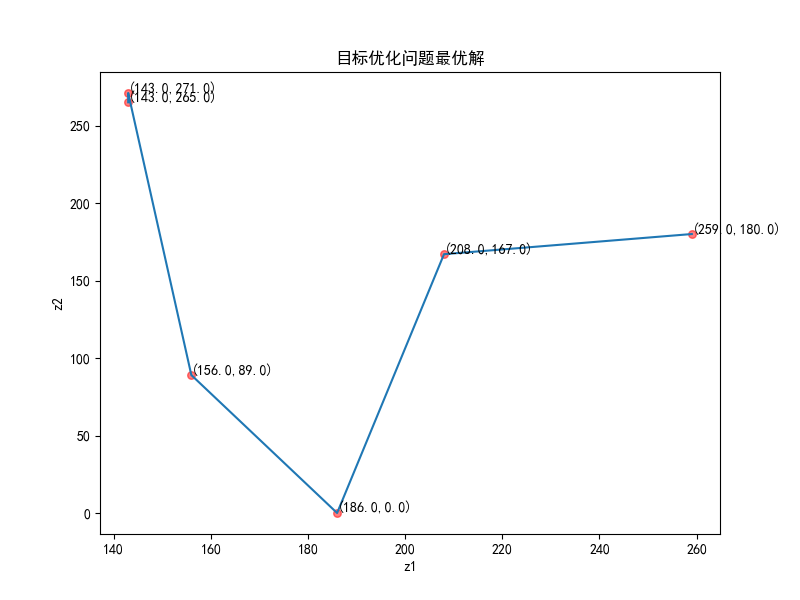
\includegraphics[width=0.4\textwidth]{figs/chap04/myplot.png}
    \caption{求解过程迭代图}
    \label{fig44}
\end{figure}

在迭代到一定程度后该算法不再收敛。选择一个可行解,以平均队列长度为评价指标与原有方法比较。

\subsection{实验与分析}

由统计结果可以得到公交站这一排队系统的几个特征:

平均到达率:$$\lambda \approx 1.56$$ 

平均等待时间:4.30(min)

平均服务率:$$\mu = 1/4.30 \approx 0.23$$

系统的服务强度:$$\rho = 6.67 $$

因为服务强度远远大于1,说明系统的服务能力不足以应对到达率,系统会出现排队现象,
排队长度可能会不断增加。如果希望系统稳定运行,需要增加服务能力或降低到达率。通过实际分析,系统在高峰时期更容易产生阻塞,
可以在高峰时期采用大小区间的方案解决这一问题。分别取t=60、120、180、240进行模拟,可以得到原始方案中用户到达服务图:
\begin{figure}[htbp]
    \center
    \subfigure[t=60]{\label{601}
    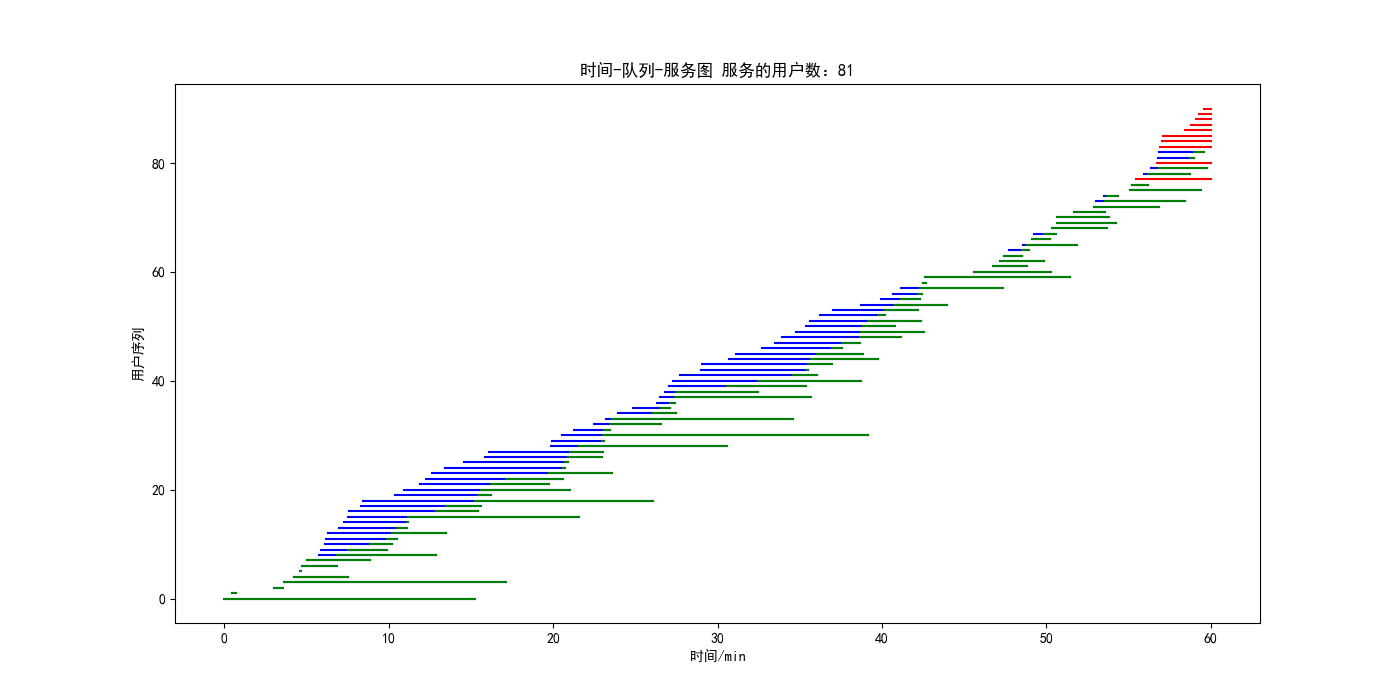
\includegraphics[width=0.4\textwidth]{figs/chap03/601.png}
    }\subfigure[t=120]{\label{1201}
    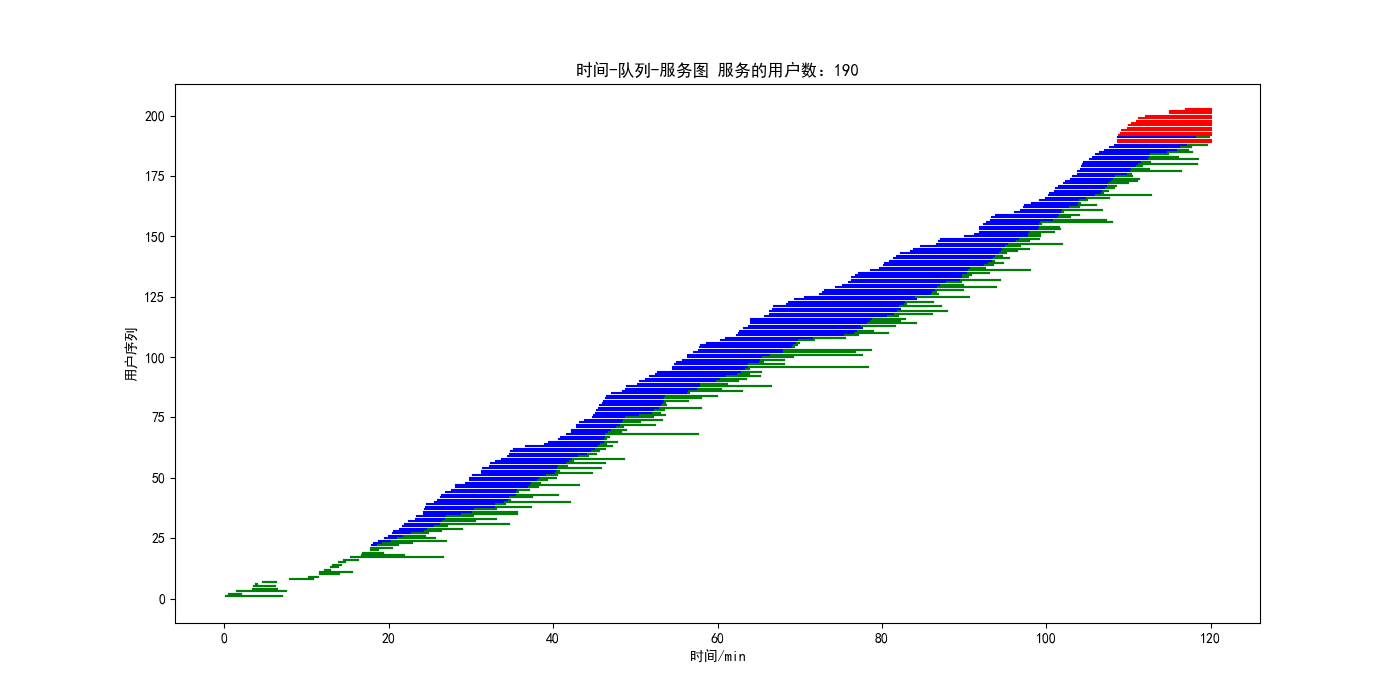
\includegraphics[width=0.4\textwidth]{figs/chap03/1201.png}
    }
    \\
    \subfigure[t=180]{\label{1801}
    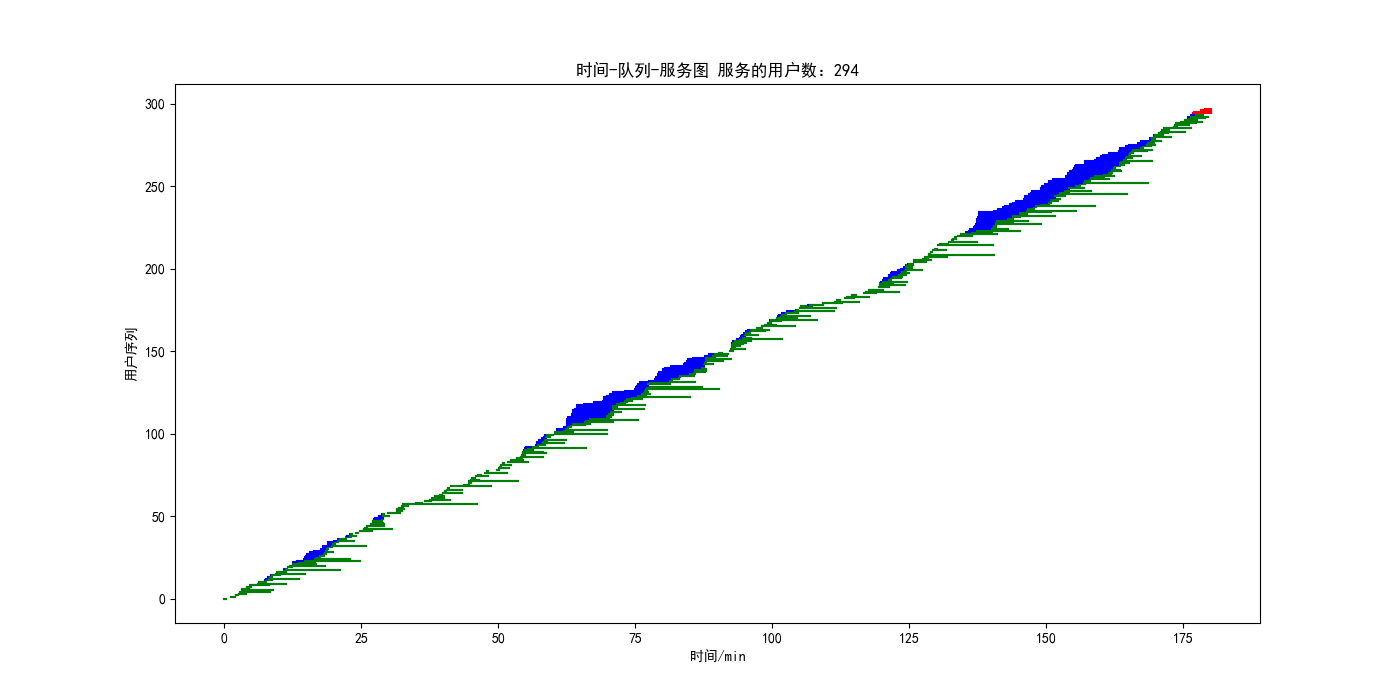
\includegraphics[width=0.4\textwidth]{figs/chap03/1801.png}
    }\subfigure[t=240]{\label{2401}
    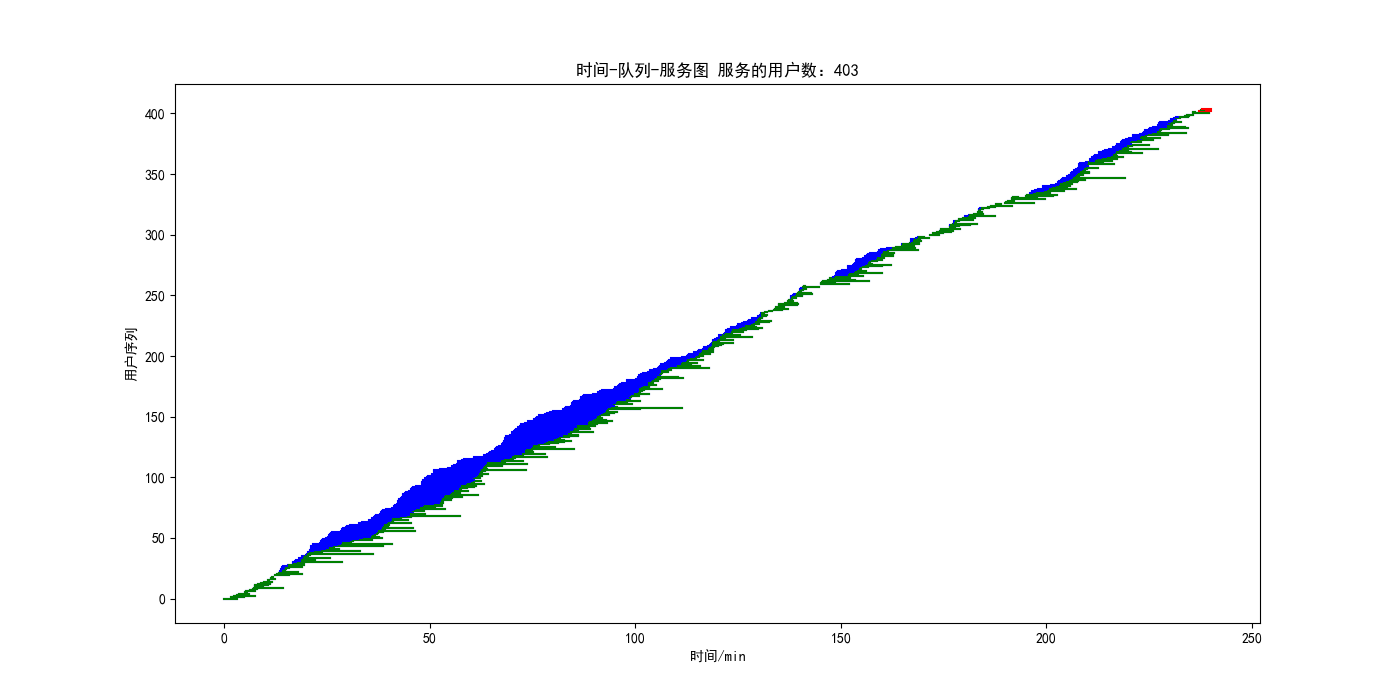
\includegraphics[width=0.4\textwidth]{figs/chap03/2401.png}
    }
    \caption{系统时间-队列-服务图}\label{fig34}
\end{figure}


系统的时间-队列长度图:
\begin{figure}[htbp]
    \center
    \subfigure[t=60]{\label{602}
    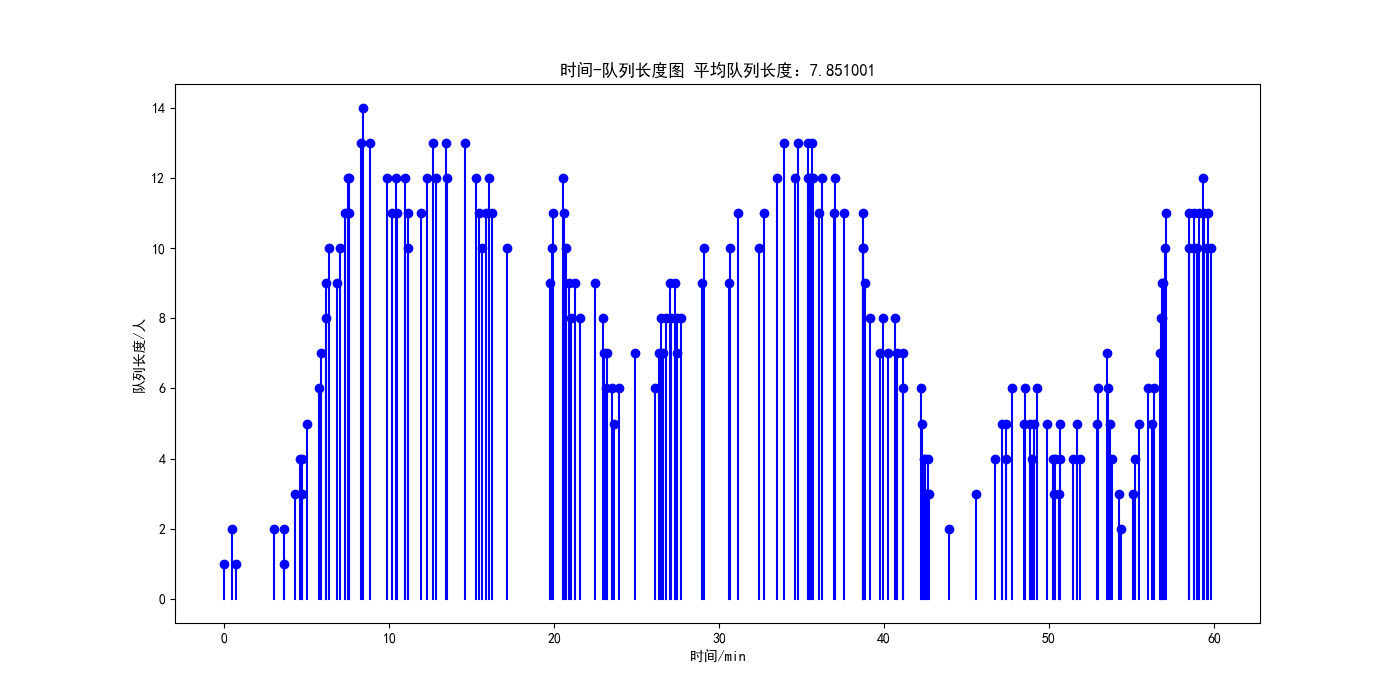
\includegraphics[width=0.4\textwidth]{figs/chap03/602.png}
    }\subfigure[t=120]{\label{1202}
    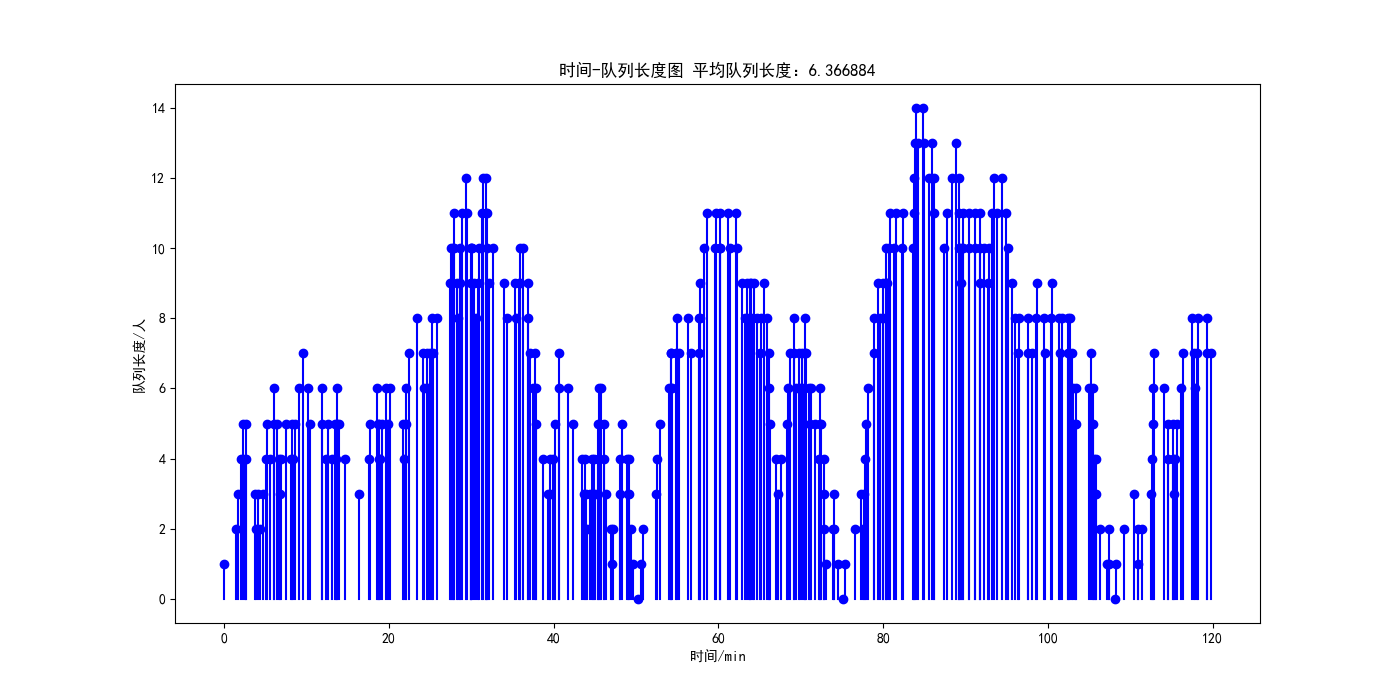
\includegraphics[width=0.4\textwidth]{figs/chap03/1202.png}
    }
    \\
    \subfigure[t=180]{\label{1802}
    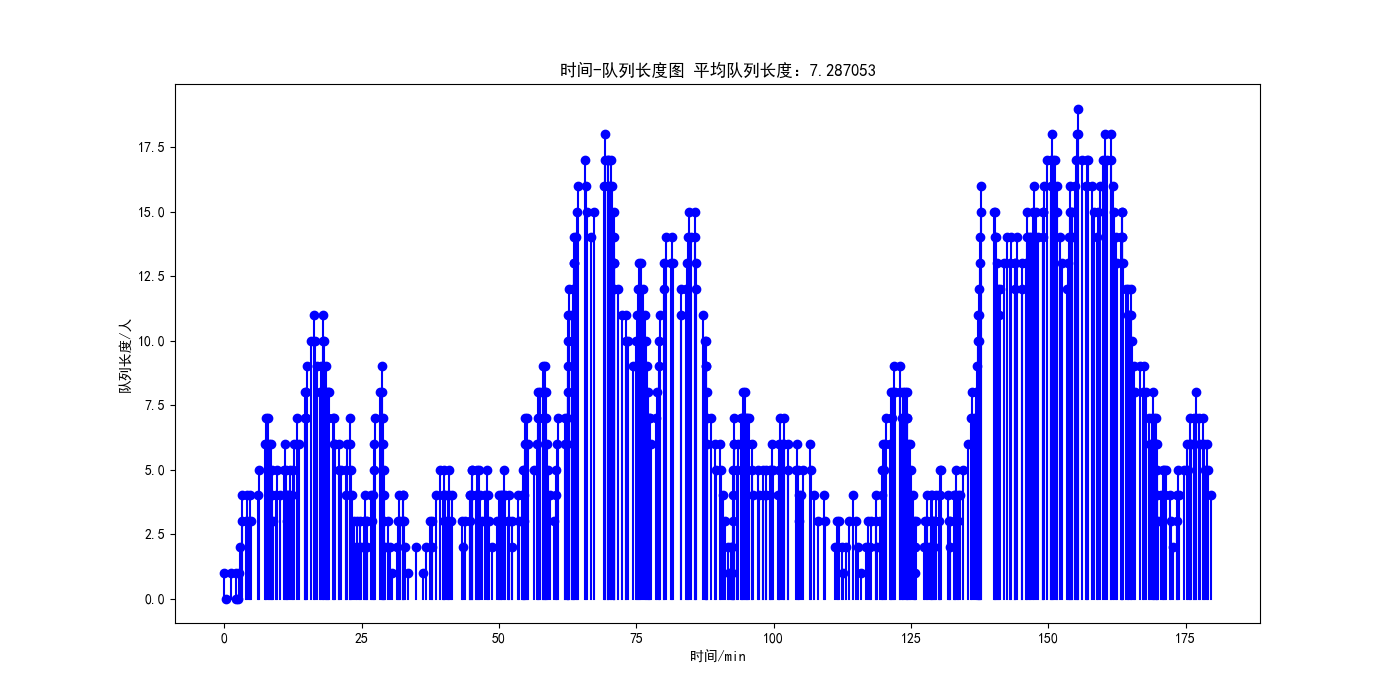
\includegraphics[width=0.4\textwidth]{figs/chap03/1802.png}
    }\subfigure[t=240]{\label{2402}
    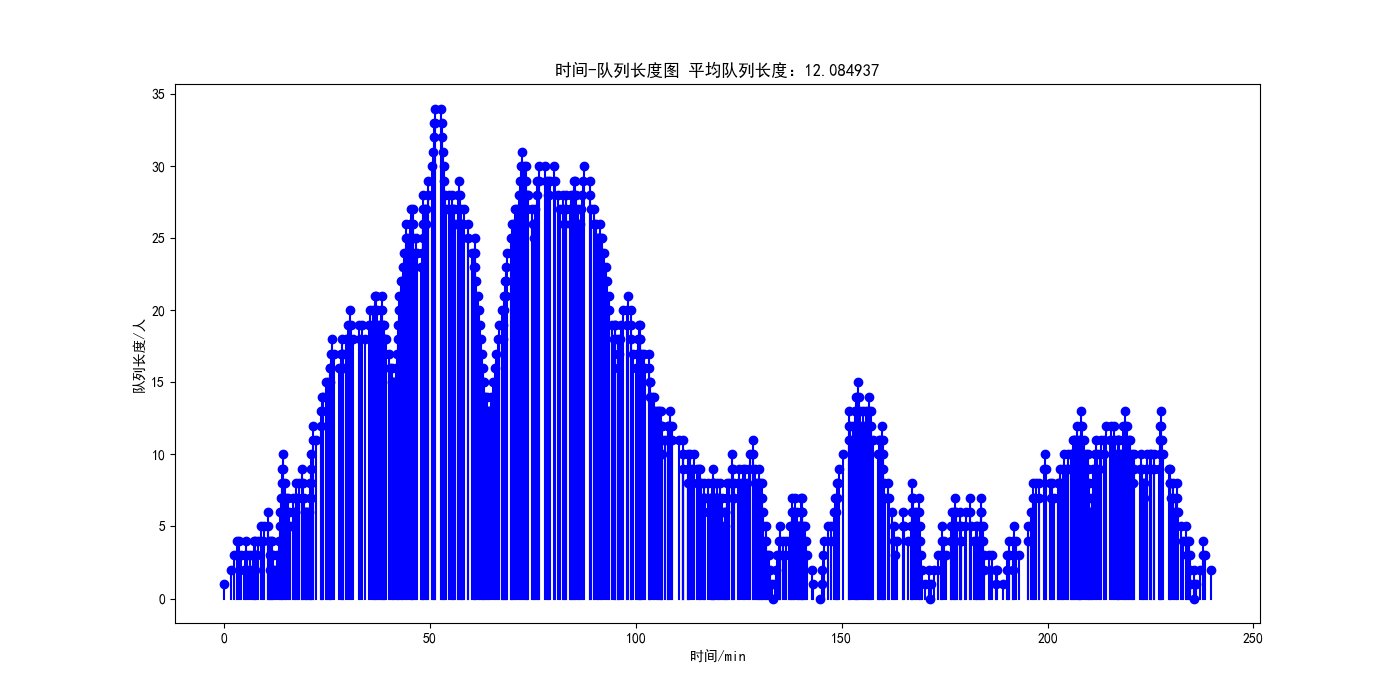
\includegraphics[width=0.4\textwidth]{figs/chap03/2402.png}
    }
    \caption{系统时间-队列长度图}\label{fig35}
\end{figure}

系统的时间-等待时间图:
\begin{figure}[htbp]
    \center
    \subfigure[t=60]{\label{603}
    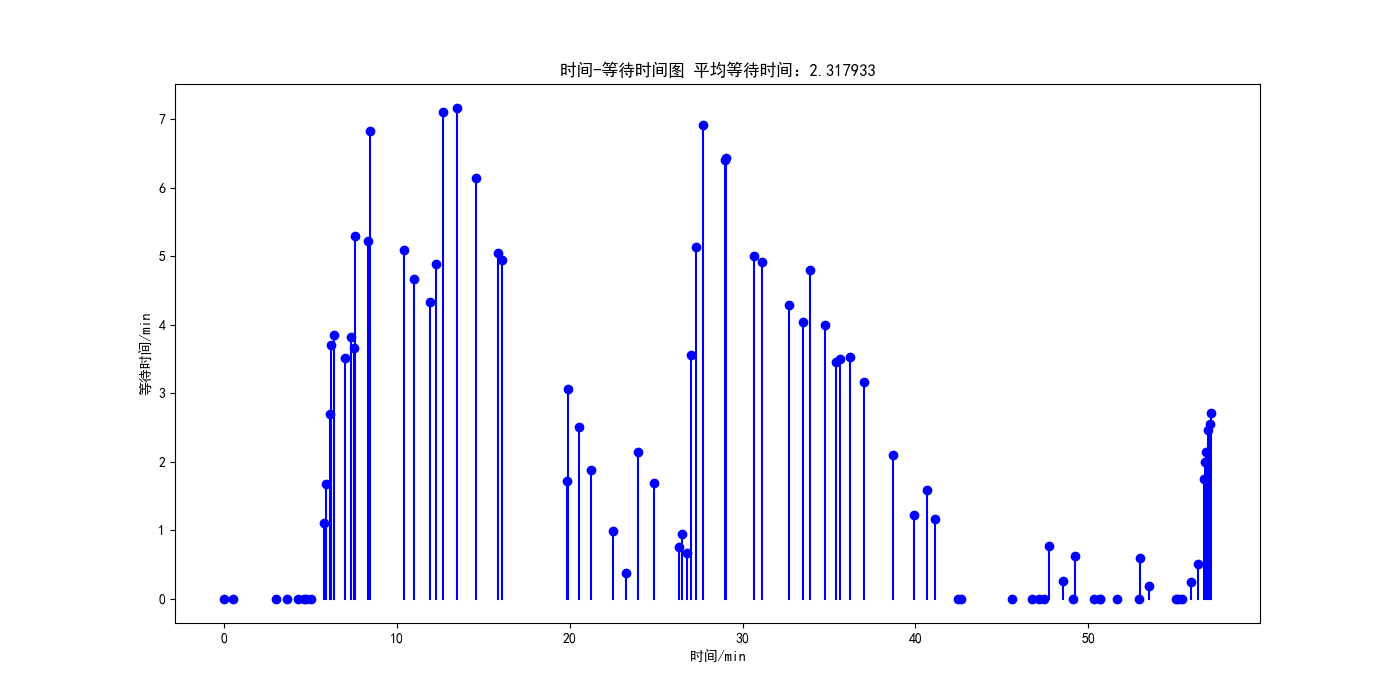
\includegraphics[width=0.45\textwidth]{figs/chap03/603.png}
    }\subfigure[t=120]{\label{1203}
    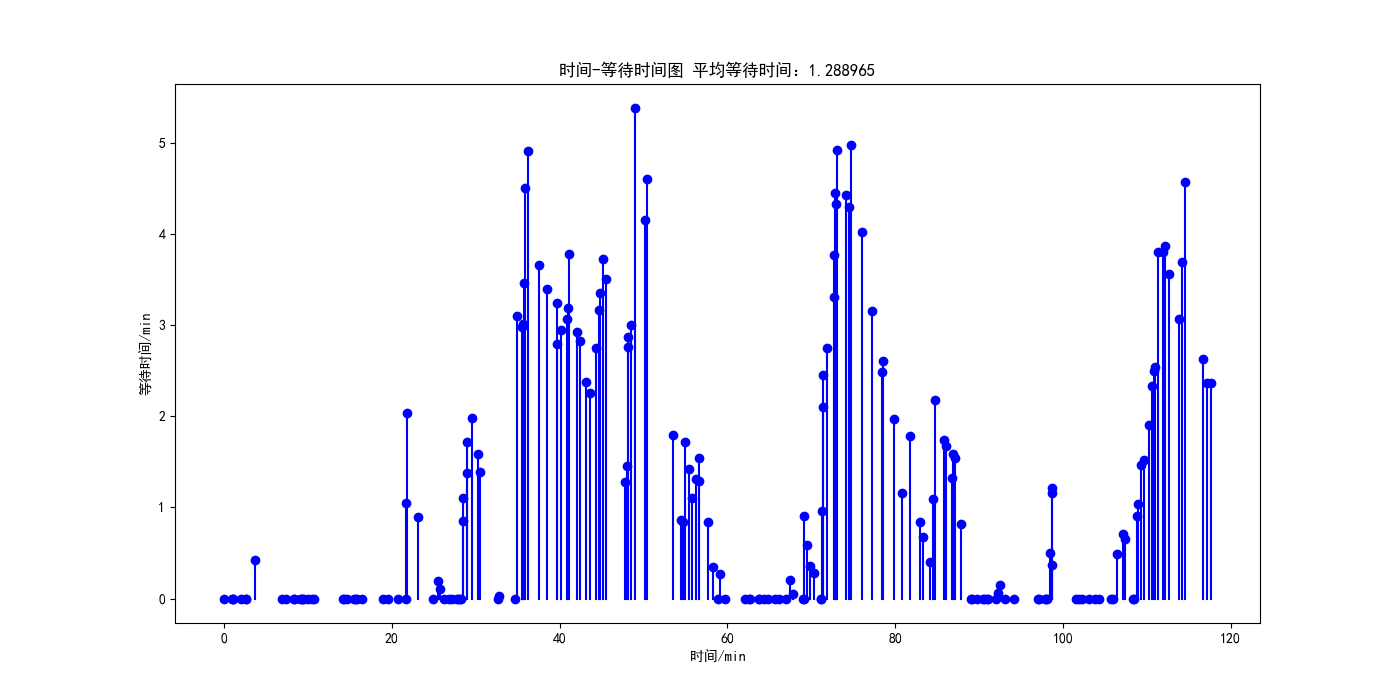
\includegraphics[width=0.45\textwidth]{figs/chap03/1203.png}
    }
    \\
    \subfigure[t=180]{\label{1803}
    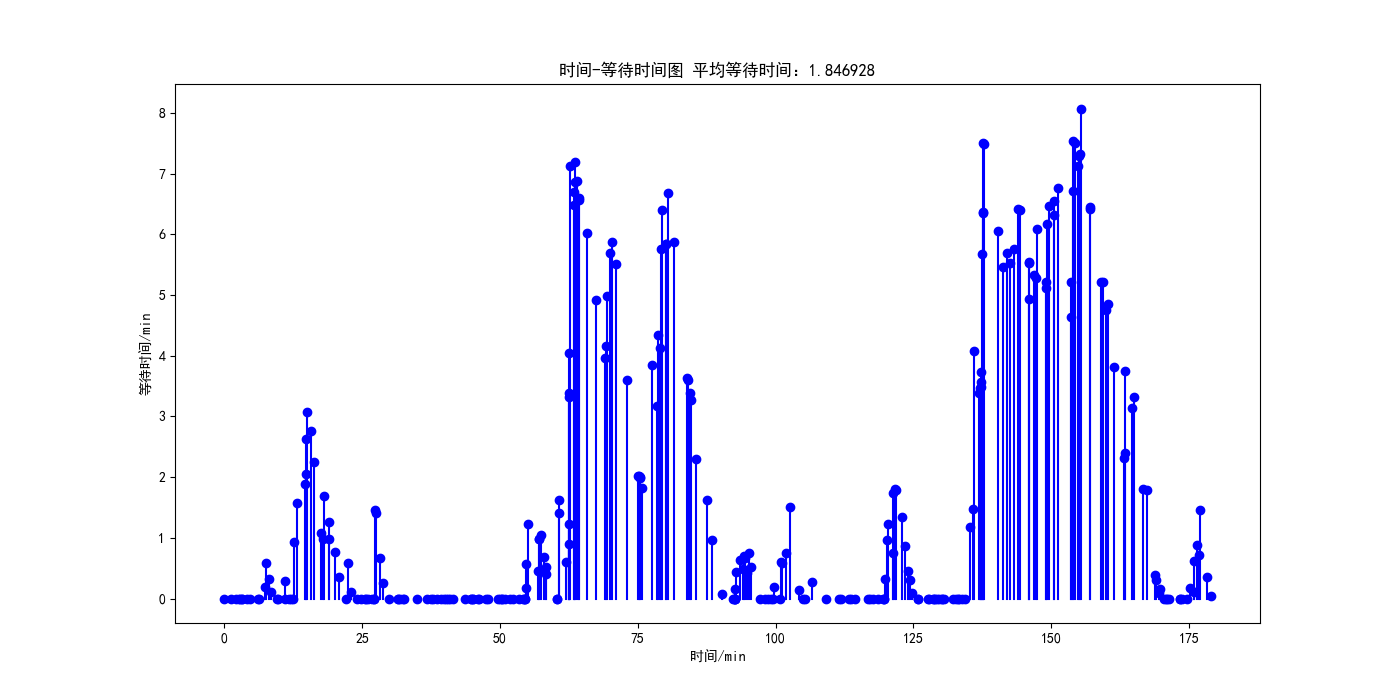
\includegraphics[width=0.45\textwidth]{figs/chap03/1803.png}
    }\subfigure[t=240]{\label{2403}
    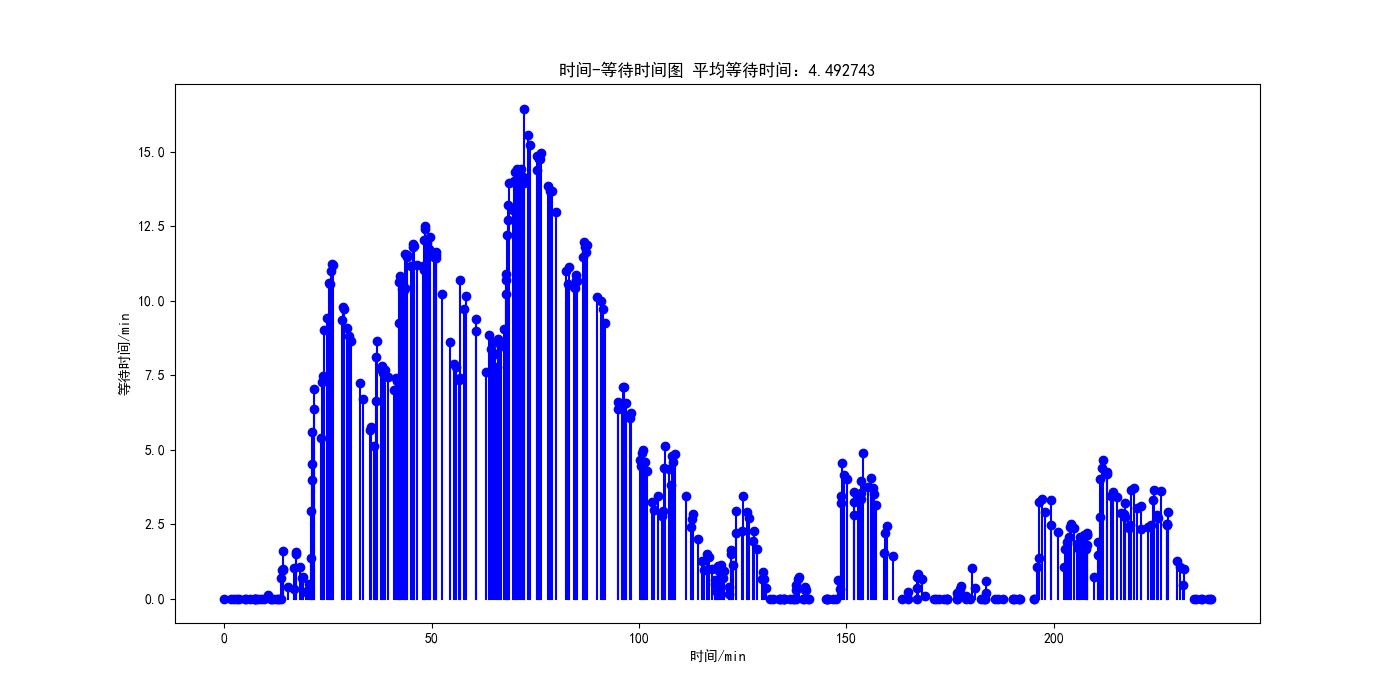
\includegraphics[width=0.45\textwidth]{figs/chap03/2403.png}
    }
    \caption{系统时间-等待时间图}\label{fig36}
\end{figure}

选择一个最优解,得到如下运行图。
\begin{figure}[htbp!]
    \centering
    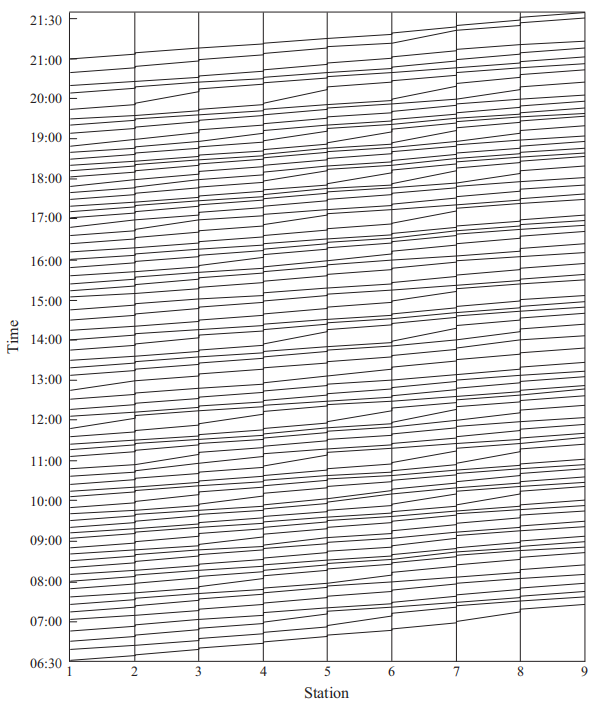
\includegraphics[width=0.4\textwidth]{figs/chap04/time.png}
    \caption{优化后的运行图}
    \label{fig45}
\end{figure}

在该实验中,按照3.2中介绍的模型构建方法使用Gurobi搭建模型。
通过迭代计算,在迭代次数超过180后模型开始不收敛。在不考虑大小区间的情况下,所得的可行解可以得到一个较好的方案。

使用表~\ref{table_1}~中的数据,通过图~\ref{fig32}~中的关系重新计算指标,使用大小区间方案处理后可以得到:
$$
\rho = 0.84
$$

对该系统进行模拟结果如下:
\begin{figure}[htbp!]
    \center
    \subfigure[系统时间-队列-服务图]{\label{1}
    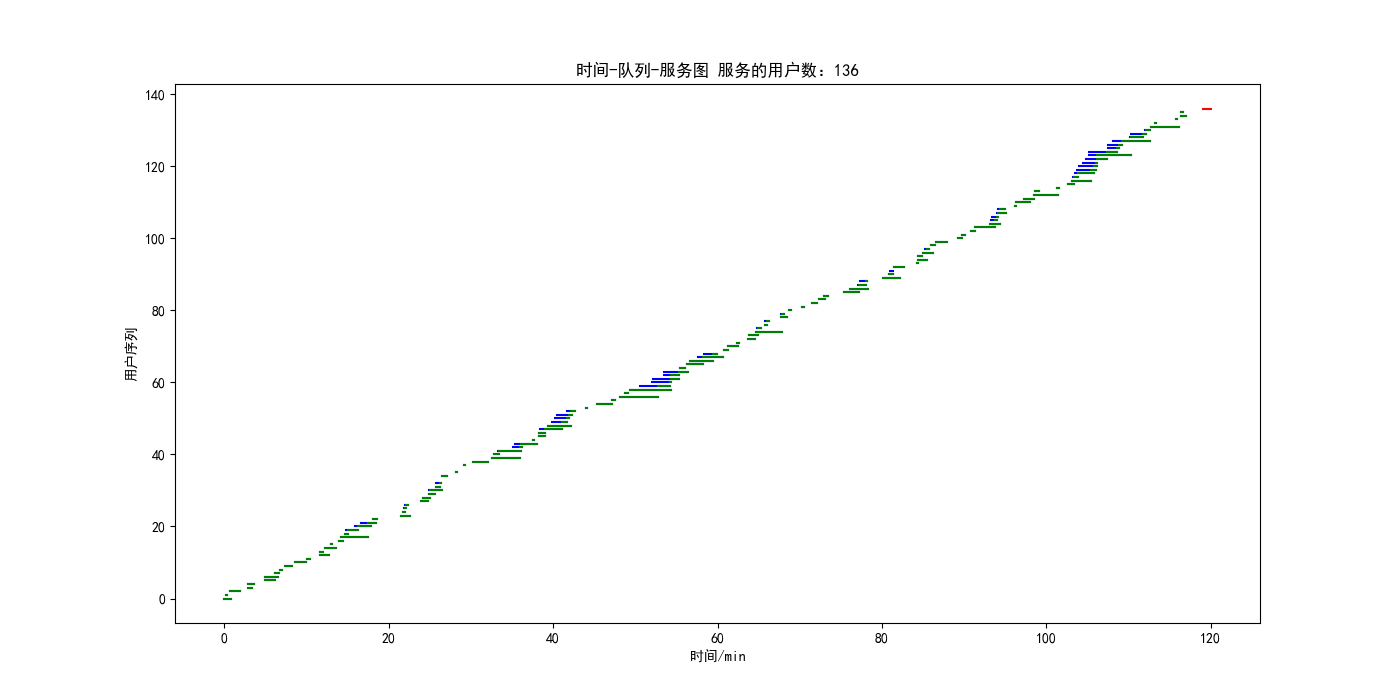
\includegraphics[width=0.5\textwidth]{figs/chap04/01.png}
    }
    \\
    \subfigure[系统时间-队列长度图]{\label{2}
    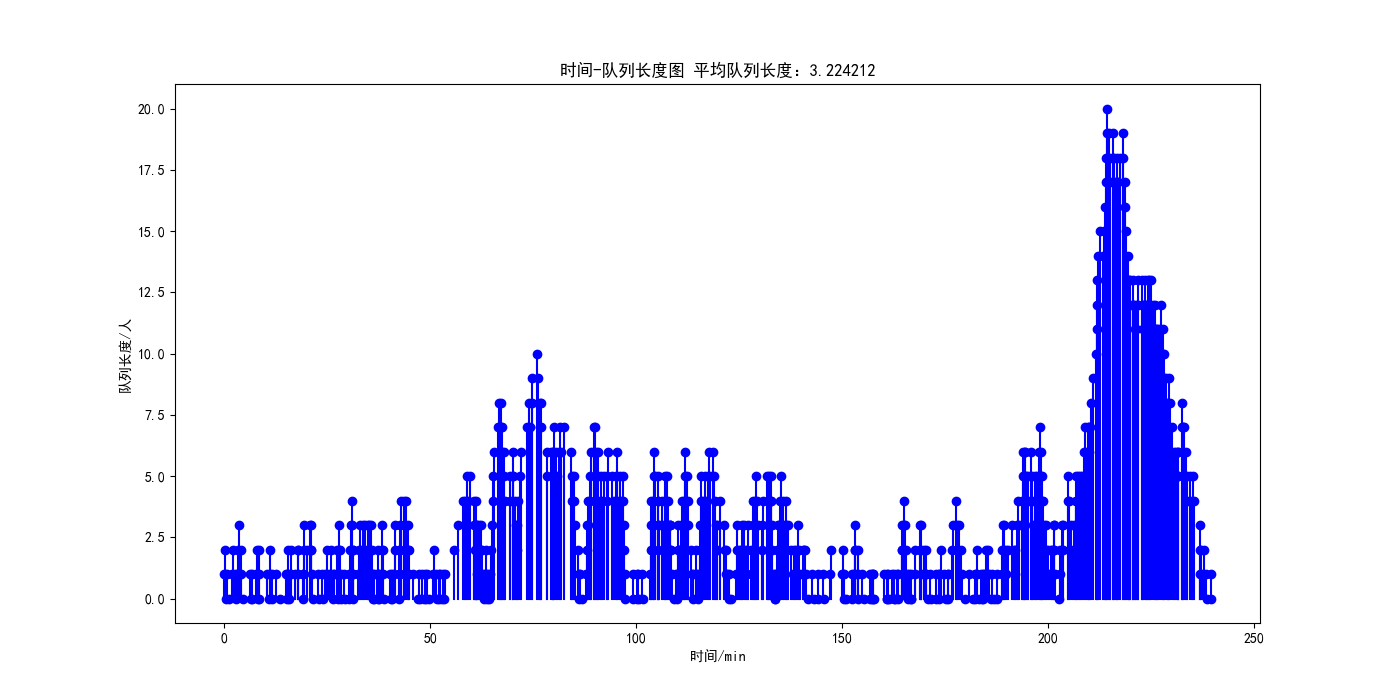
\includegraphics[width=0.5\textwidth]{figs/chap04/02.png}
    }
    \\
    \subfigure[系统时间-等待时间图]{\label{3}
    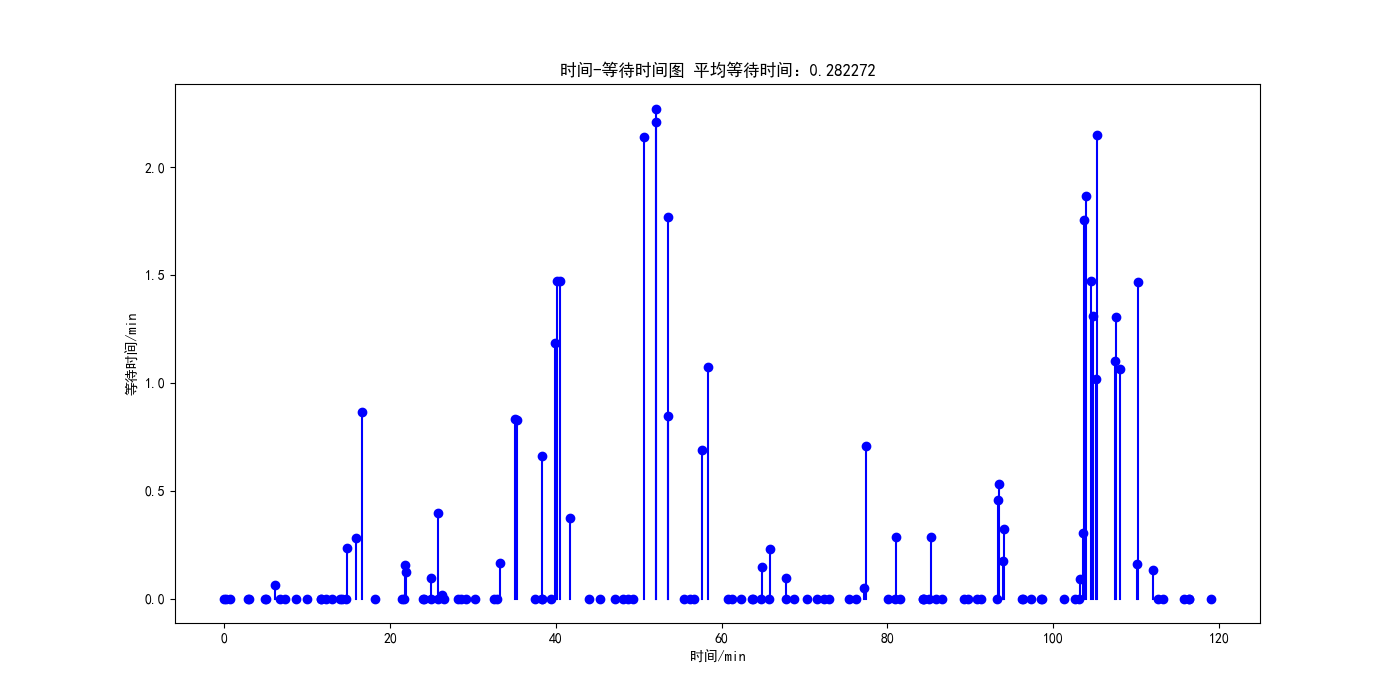
\includegraphics[width=0.5\textwidth]{figs/chap04/03.png}
    }
    \caption{优化后系统的模拟结果}\label{fig47}
\end{figure}
